\documentclass[../main.tex]{subfiles}
 
\begin{document}

\section{Tuesday}

You knew you had to check-in at 9 am for your first of two shifts today, so you were sure to get back the night before and get plenty of sleep. Nonetheless, you push it when it comes to making it your first schedule so that you can get some extra sleep. Although you are supposed to show up for staging in the SV office 30 minutes before your shift, you end up catching your Team Leader mid flight with a group of volunteers being lead into Experience Hall for their placements. You check in and are rightfully chastized for showing up when you do. A 15 minute Uber ride with a driver who got lost, followed by a long line at the Hilton Starbucks next door made you late. You could have been responsible and showed up for your back to back shift on time, but then you would have arrived at 3 pm without having eaten breakfast.

Where you are placed happens to be another booth in E-tech that is run by the same Japanese lab with the Haptic finger apparatus that you tried on Monday. These fellows do not speak English and you are unimpressed by a keyboard that vibrates being billed as a high quality instrument for musicians. You have seen hungover undergraduates do better than this in a weekend in the lab back at school, and you are annoyed that their advertisement materials have typos and their equipment constantly requires intervention from one of the students restore its functionality. It is not the case that you are simply being too hard on these guys: several attendees have walked pressed a key or two and walked off, and more than one walked away without trying the device after hearing you explain that it is a keyboard which speakers in the keys which help give the sensation of various percussion instruments as you press each key. This emerging tech strikes you as clumsy and poorly thought out. Its obvious that the students asociated with the lab have simply taken their passion for music and what hardware knowledge they had and put the two together to create an instrument that ticks the "haptic" checkbox. You resent representing a product that people so clearly do not care about. For all the hype surrounding SIGGRAPH, this stuff just seems silly. You would like to say that everything at SIGGRAPH was just absolutely mind blowing, but your experience in Experience Hall once again suggests that only certain parts of the convention are worth investing your time. Then again, perhaps a keyboard that vibrates is more intersting to folks encountering it for 30 seconds than it is to someone who must explain what it is for 3 hours straight. The fact that most of the novelty to be found in Experience Hall can wear off so quickly is indicative of what one ought to concentrate on. Probably the production sessions, even over the technical talks.

Following this shift, you then have another stressful shift working with Rolland, during which you handle a constant stream of requests to print emailed images onto tote bags. You gain an appreciation for what working in retail must be like and are humbled by how difficult you found the 3 hour rush to process the print request with attendees standing behind you, managing your work as you fumble around with Adobe Illustrator templates. Frustration builds as requests pile up and for some reason the gosh darn mask won't clip the images. One kind attendee helps you fix the layer hierarchy to get you moving again. To your left another SV does a similar job, except for emailed images meant to be printed on iPhone cases. You feel badly at your own behavior when a tiny crack appears in your dike of patience after a lot of nagging from one attendee in particular. This lady practically throws a fit as you struggle to positon her photo on your screen, you simply scoot your chair back and point at your keyboard, gesturing for her to draw up her free design as she wishes. When your shift is over, you realize how much you have taken for granted a life free of working in \textit{retail}, with \textit{customers}.

During the afternoon you manage to catch a wonderful talk in Room 207 D, where companies like Autodesk and Nvidia present various talks, some of which have been selected as "Best of" talks after being presented at other gatherings. The speaker is Matt Silverman, a designer, animator, director, and entrepreneur who now runs the scrappy company Swordfish out of San Francisco. Swordfish is unique in its completely cloud-based rendering workflow. The talk discusses how Swordfish uses a Google Cloud Platform to pay for large amounts of computer power on an as-needed basis to complete their commercial work. The talk covers how Matt grew his company by carefully buying company only as new employees came onboard, picking up Mac Pro desktop computers off of craigslist to amass a small in house renderfarm while choosing when to pay a few thousands of dollars here or their to spool up servers in the cloud which crunch thorugh thier renders---all without the tremendous upfront investment made by other larger companies in hardware. You see several commercials he has made and are treated to a well told story of the arc of his company.

\begin{figure}[h!]
	\centering
	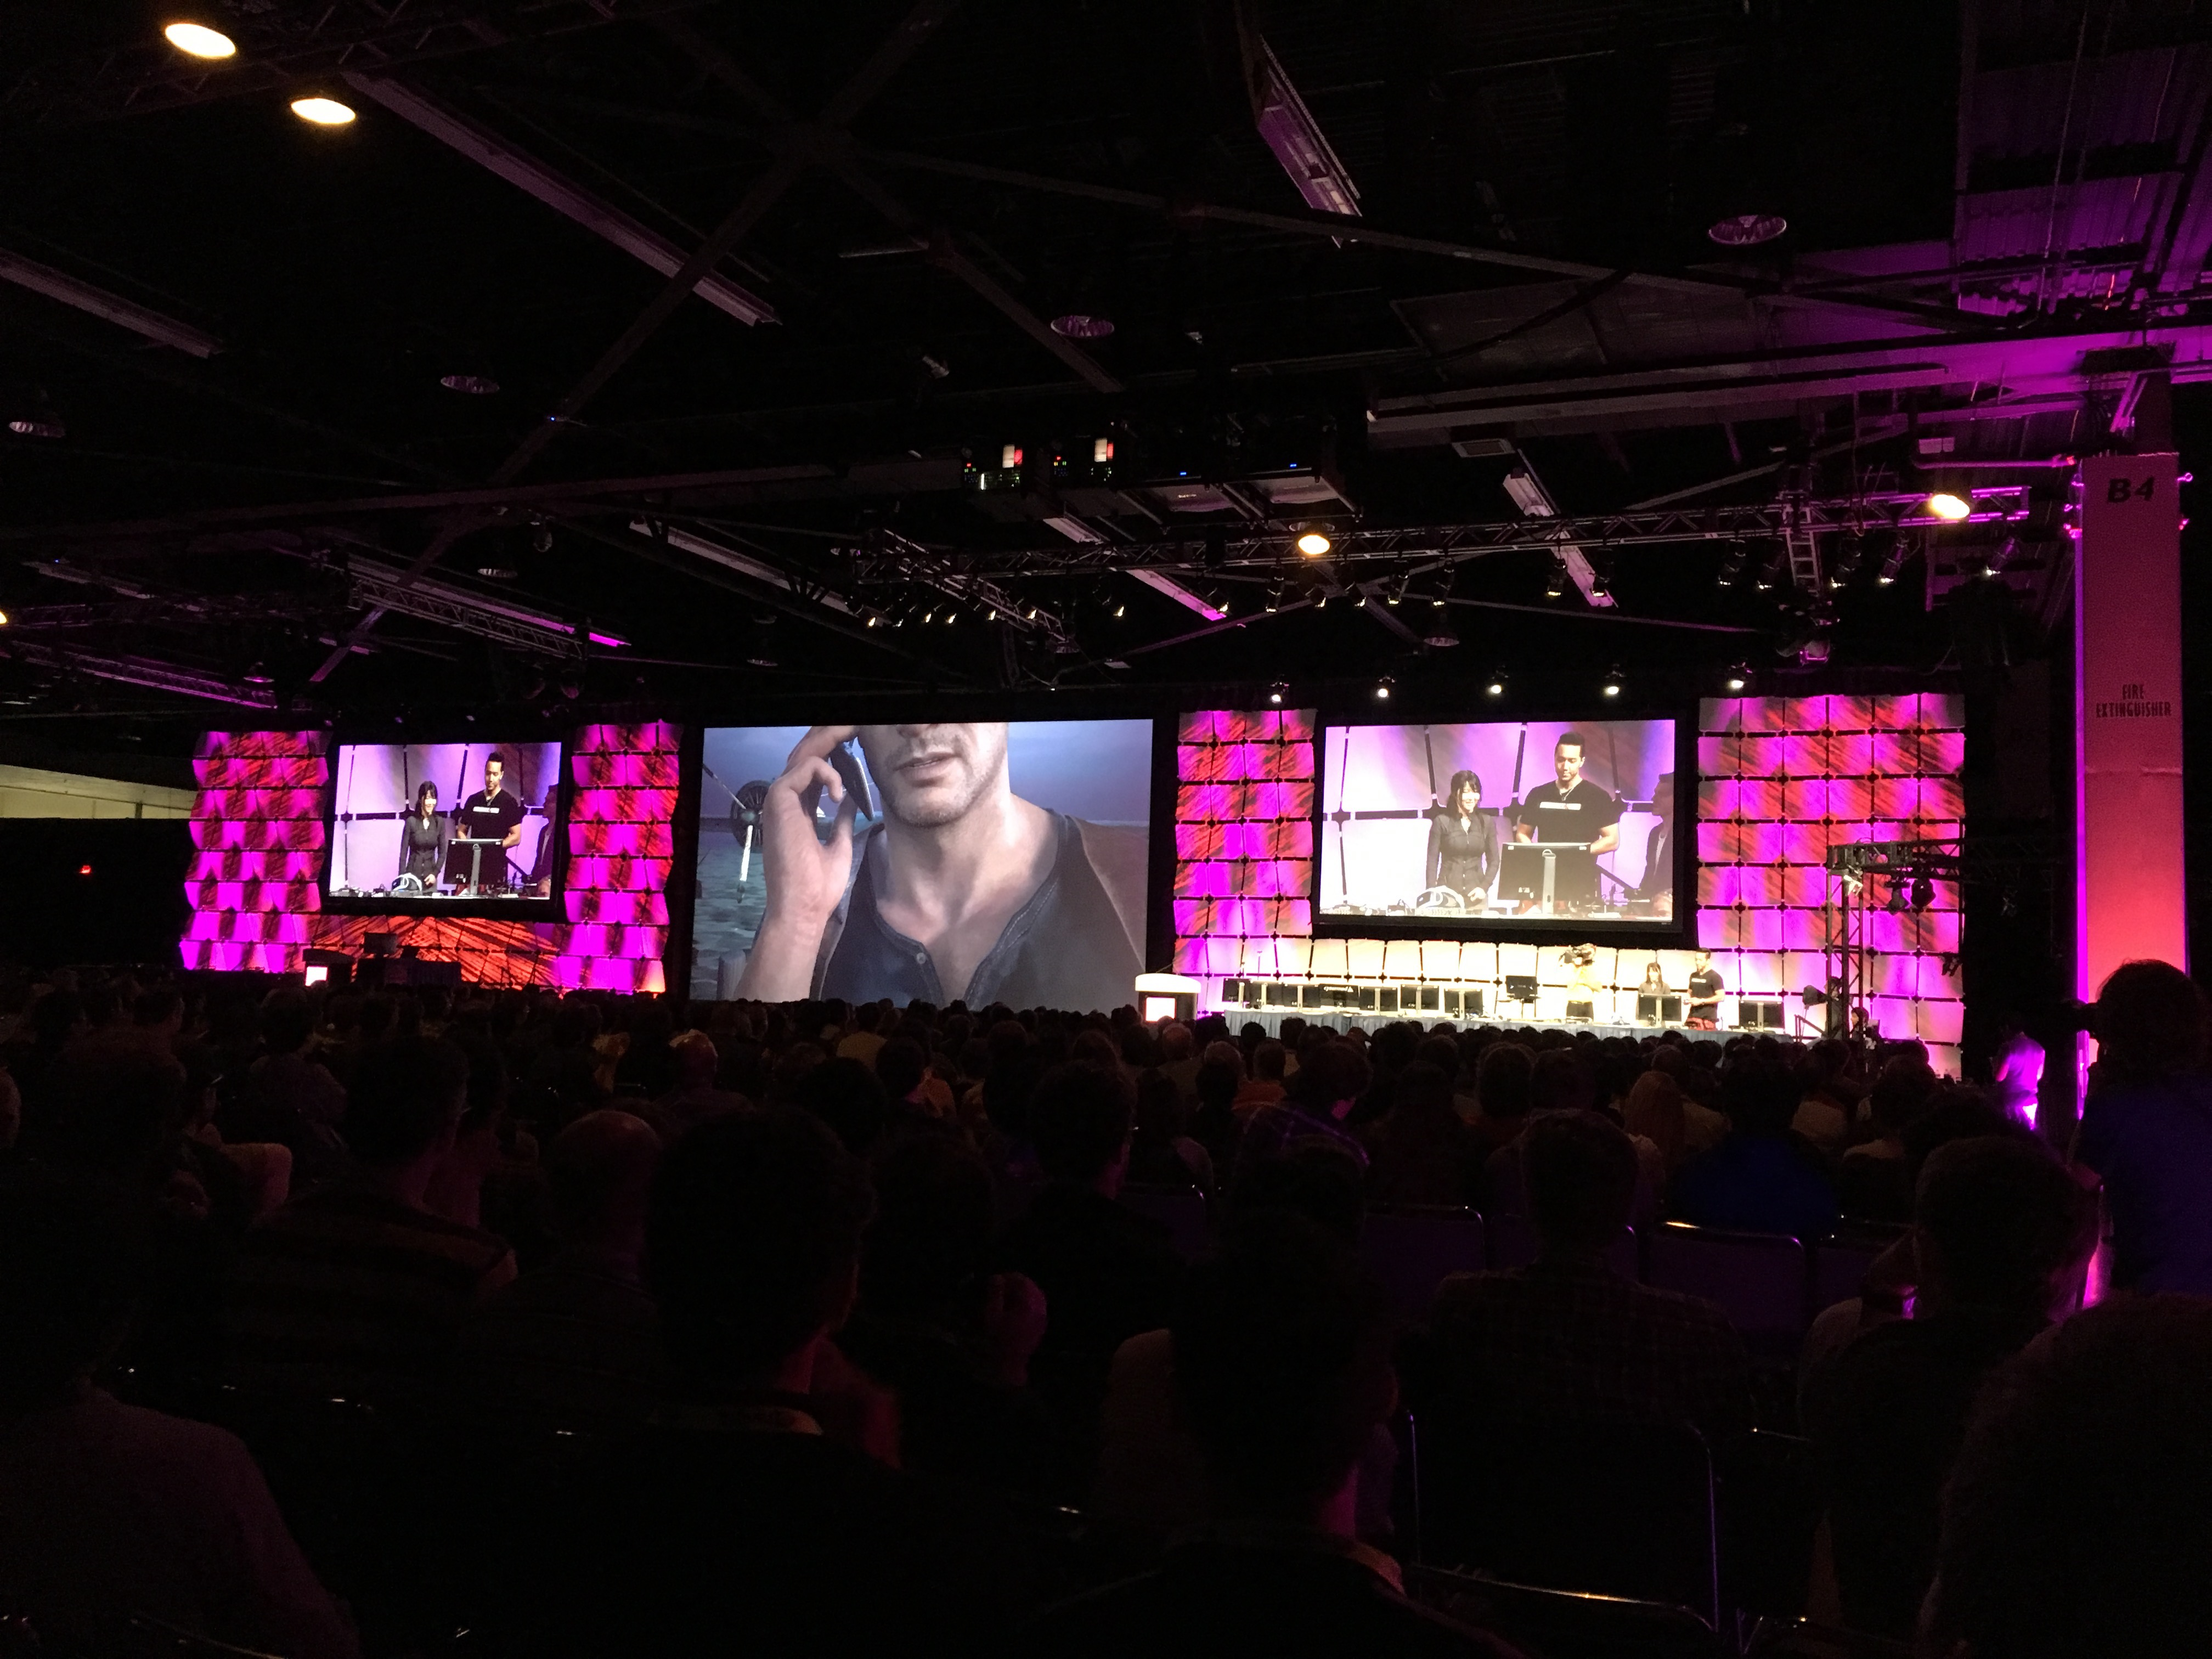
\includegraphics[width=\textwidth]{real-time_live}
	\caption*{Real-time Live. "Look at how we render Drake's chest hair."}
\end{figure}

Later in the evening you drop in to see \textit{Real-Time Live} in Hall B. 

\end{document}